\documentclass[12pt,a4paper]{article}
\usepackage[utf8]{inputenc}
\usepackage[T1]{fontenc}
\usepackage[french]{babel}
\usepackage{graphicx}
\usepackage{hyperref}
\usepackage{geometry}
\geometry{a4paper, margin=2.5cm}
\usepackage{listings}
\usepackage{xcolor}
\usepackage{caption}
\usepackage{float}

% Configuration pour les blocs de code Java
\lstset{
    language=Java,
    backgroundcolor=\color{lightgray!10},   
    basicstyle=\ttfamily\footnotesize,
    keywordstyle=\color{blue}\bfseries,
    stringstyle=\color{red},
    commentstyle=\color{green!60!black}\itshape,
    breaklines=true,                 
    captionpos=b,                    
    keepspaces=true,                 
    numbers=left,                    
    numbersep=5pt,                  
    showspaces=false,                
    showstringspaces=false,
    showtabs=false,                  
    tabsize=2,
    frame=single,
    rulecolor=\color{black!30}
}

\title{\textbf{Compte Rendu Détaillé de Projet JEE} \\ \Large Application de Gestion : \textit{Classroom CRB}}
\author{BOUSSADIA Chaabane \& BETTAHER Raed\\ \small Spécialité : IGL4}
\date{\today}

\begin{document}

\maketitle

\begin{center}
    \textit{Projet de Développement encadré par : \textbf{Mme Fourati Hend}}
\end{center}

\vspace{2cm}

\begin{abstract}
Ce rapport constitue le compte rendu détaillé du projet JEE "Classroom CRB". Il présente les architectures logique et physique de la solution mise en place avec Spring Boot, ainsi que la démarche complète suivie pour répondre à chaque question de l'énoncé. Les implémentations sont illustrées par des extraits de code pertinents et validées par des captures d'écran de notre propre machine, prouvant le bon fonctionnement des API, de l'interface utilisateur, de l'environnement Docker, ainsi que des mécanismes de sécurité avancés.
\end{abstract}

\newpage
\tableofcontents
\newpage
\listoffigures
\newpage

% =========================================================
\section{Architectures de l'Application}

Afin de garantir la robustesse et l'évolutivité de notre solution, nous avons clairement séparé l'architecture de conception (logique) de son architecture de déploiement (physique).

\subsection{Architecture Logique}
L'architecture logique repose sur le modèle MVC (Model-View-Controller) et une architecture stricte en couches (Layered Architecture).

\begin{figure}[H]
    \centering
    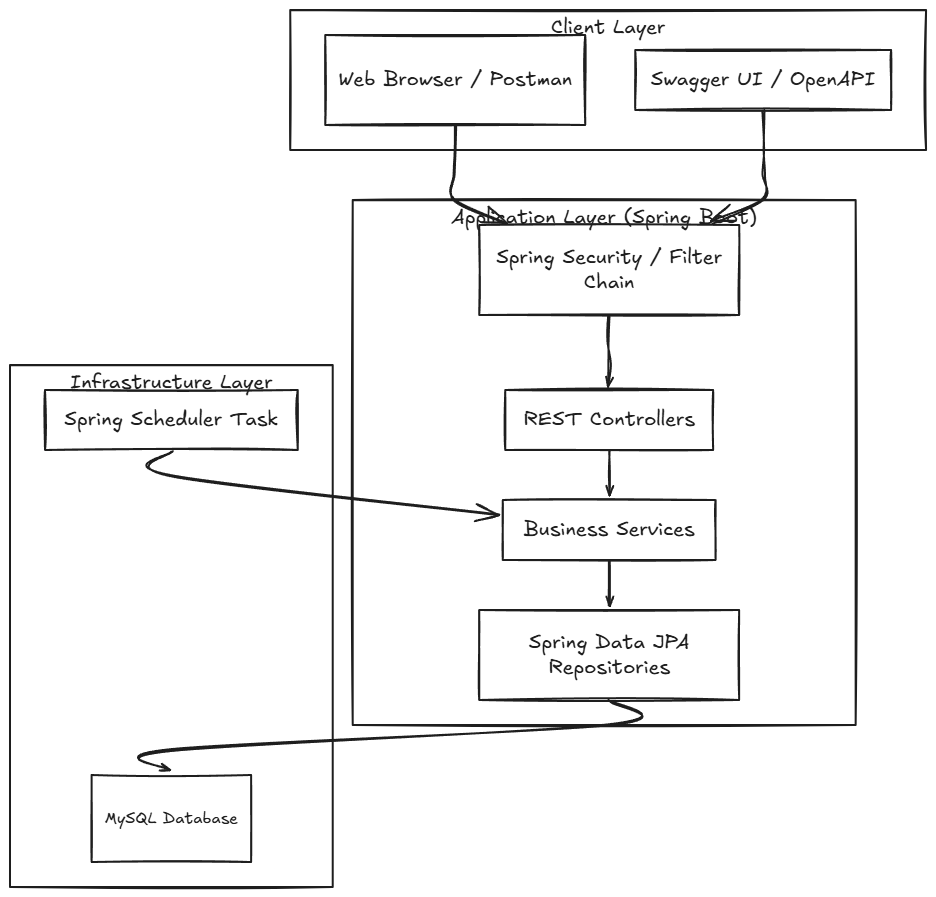
\includegraphics[width=0.9\textwidth]{../diagrams/architecture.png}
    \caption{Architecture Logique : Découpage en couches (Controller, Service, Repository)}
    \label{fig:archi_logique}
\end{figure}

Chaque requête HTTP passe par le contrôleur REST, qui délègue la logique métier complexe à la couche \texttt{Service}. L'accès aux données est ensuite géré par la couche \texttt{Repository} via Spring Data JPA. L'inversion de contrôle (IoC) de Spring s'occupe de l'injection des dépendances entre ces couches.

\subsection{Architecture Physique (Déploiement)}
L'architecture physique définit la manière dont l'application est déployée. Nous avons opté pour une approche conteneurisée.

\begin{figure}[H]
    \centering
    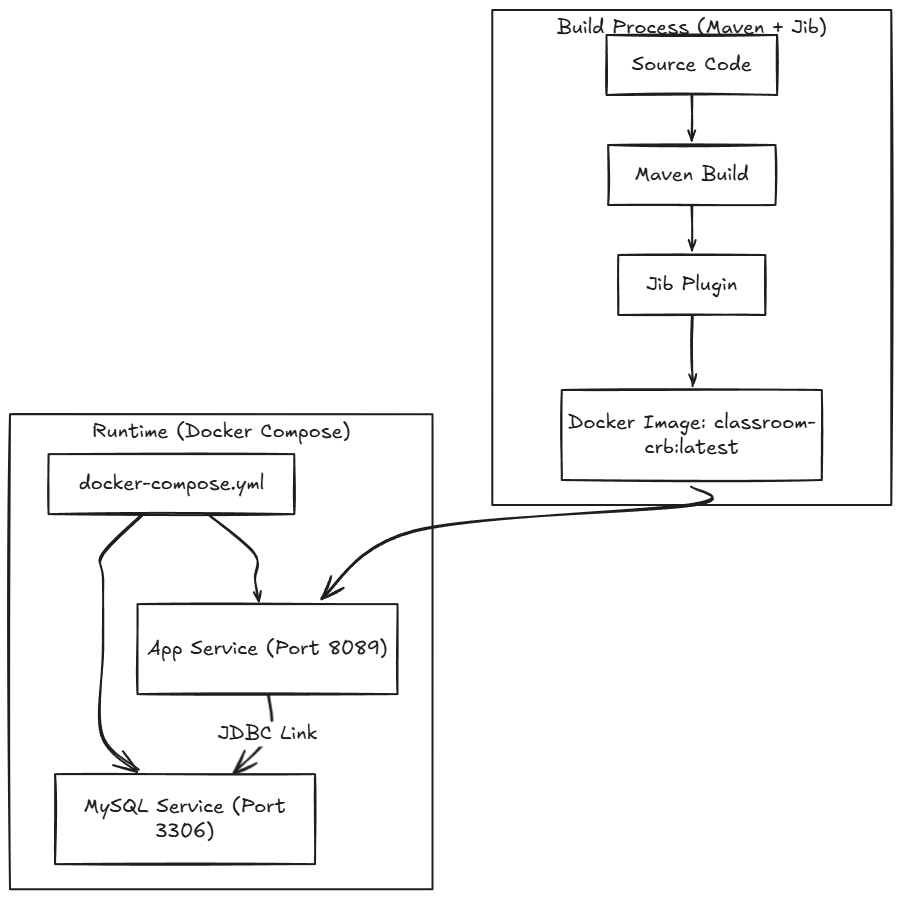
\includegraphics[width=0.85\textwidth]{../diagrams/deploy.png}
    \caption{Architecture Physique : Conteneurisation avec Jib et Docker Compose}
    \label{fig:archi_physique}
\end{figure}

L'application Spring Boot s'exécute dans un conteneur qui communique directement avec un second conteneur hébergeant la base de données MySQL via un réseau virtuel Docker.

% =========================================================
\section{Démarche et Résolution des Questions de l'Énoncé}

Cette section détaille notre démarche pour traiter séquentiellement les exigences de l'énoncé du TP.

\subsection{Question 1 : Modélisation et Entités}
\textbf{Démarche :} Nous avons créé les entités \texttt{Utilisateur}, \texttt{Classe} et \texttt{CoursClassroom} avec leurs attributs respectifs. Les relations JPA ont été établies : \texttt{@ManyToOne} entre Utilisateur et Classe, et \texttt{@OneToMany} (bidirectionnelle) entre Classe et CoursClassroom.

\begin{figure}[H]
    \centering
    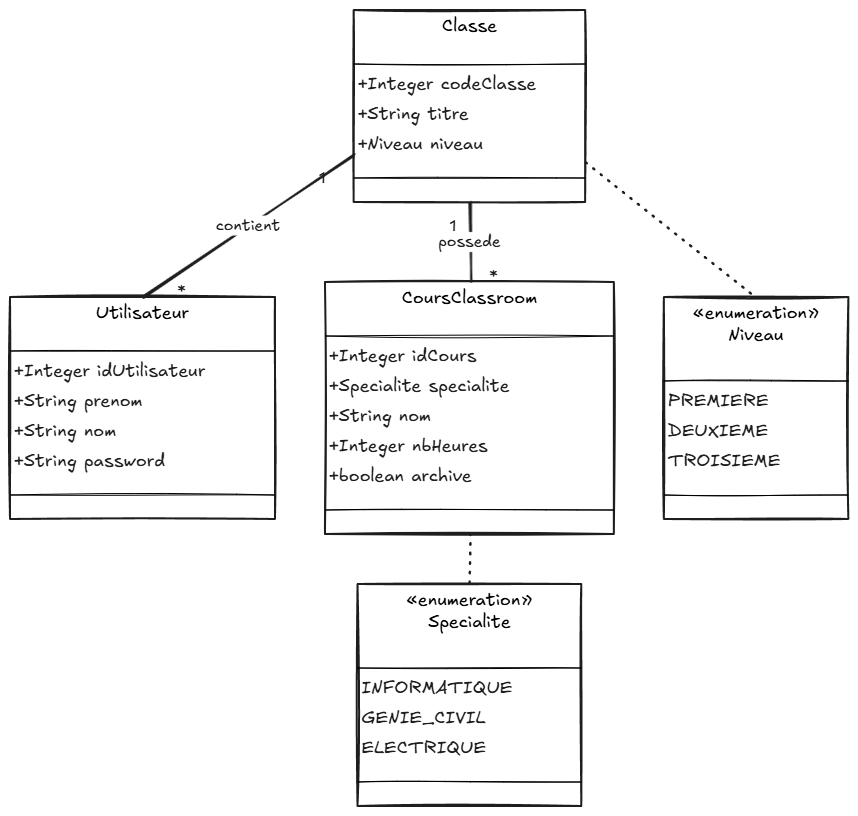
\includegraphics[width=0.8\textwidth]{../diagrams/entities.png}
    \caption{Diagramme du Modèle Conceptuel de Données (MCD)}
    \label{fig:q1_entities}
\end{figure}

\begin{figure}[H]
    \centering
    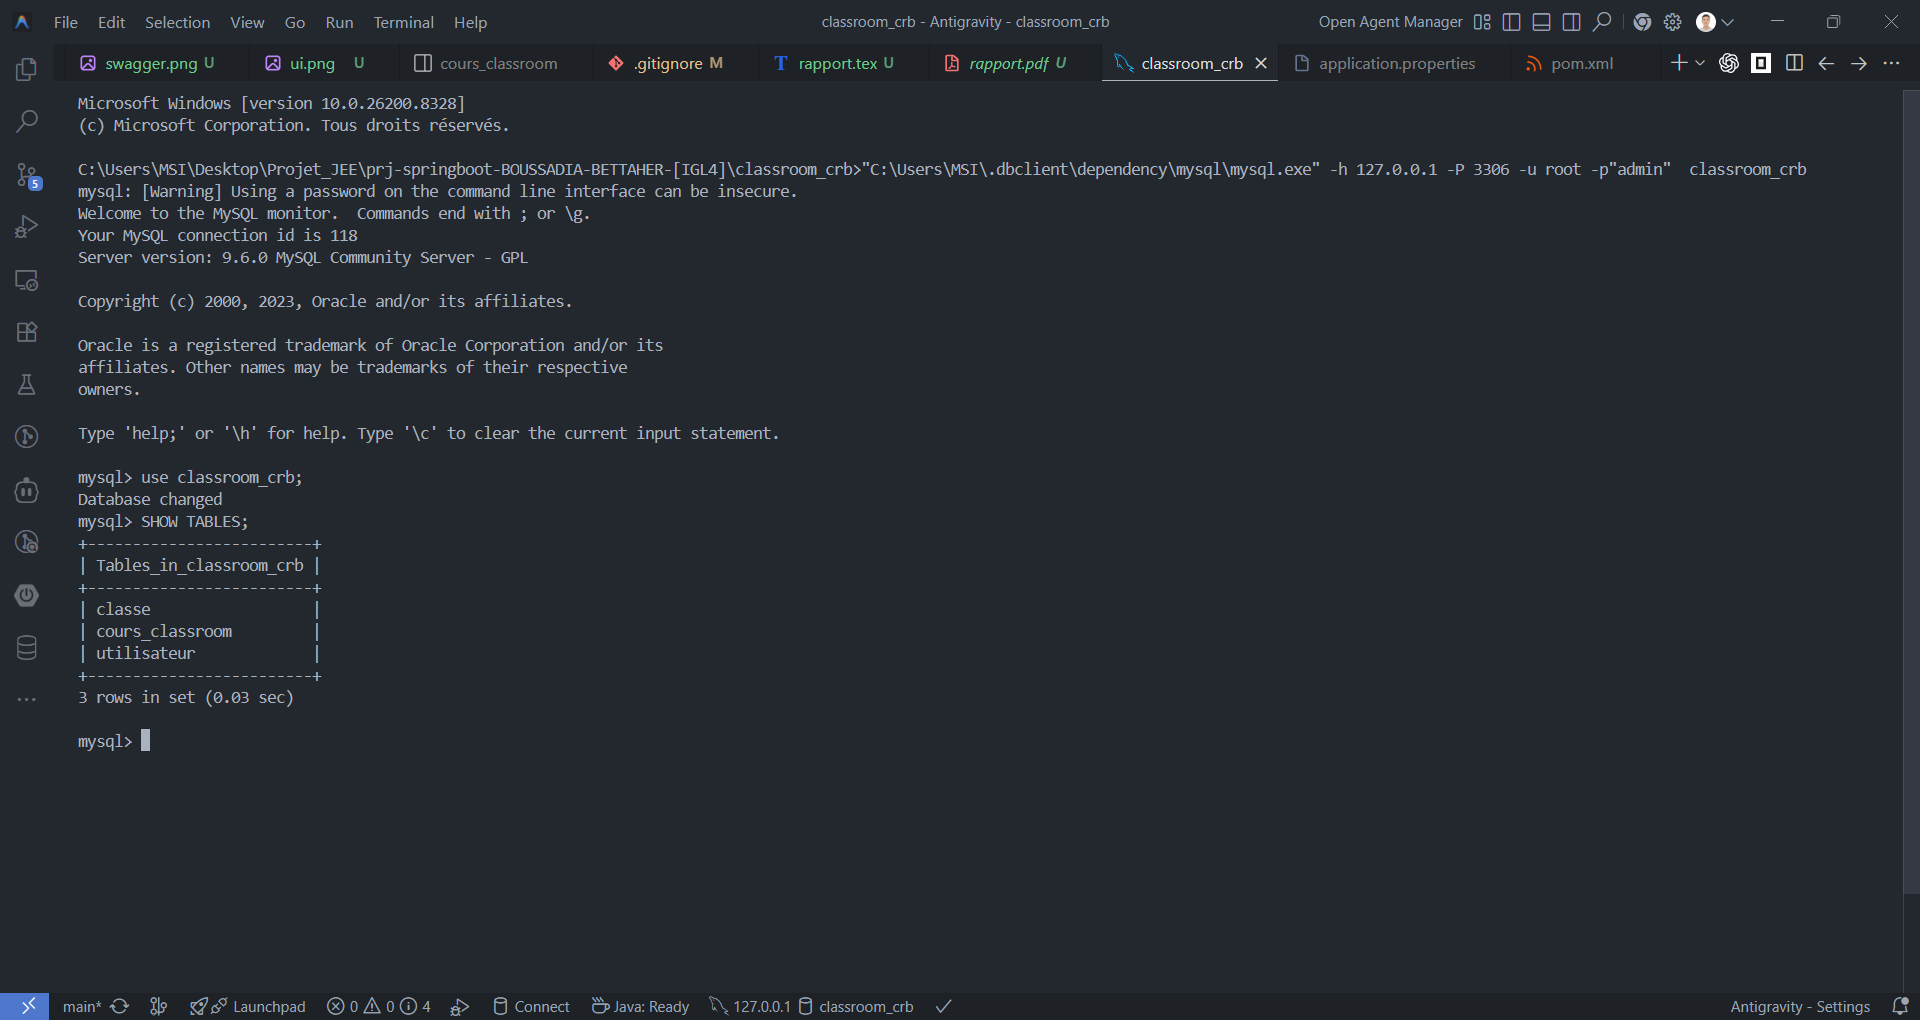
\includegraphics[width=0.9\textwidth]{../diagrams/mysql_tables.png}
    \caption{Tables créées dans la base de données (MySQL)}
\end{figure}

\subsection{Question 2 : Opérations d'Ajout (CRUD de base)}
\textbf{Démarche :} Nous avons implémenté les méthodes \texttt{ajouterUtilisateur}, \texttt{ajouterClasse} et \texttt{ajouterCoursClassroom} dans les interfaces de services respectives, puis exposé ces services via les contrôleurs REST (\texttt{@PostMapping}).

\begin{figure}[H]
    \centering
    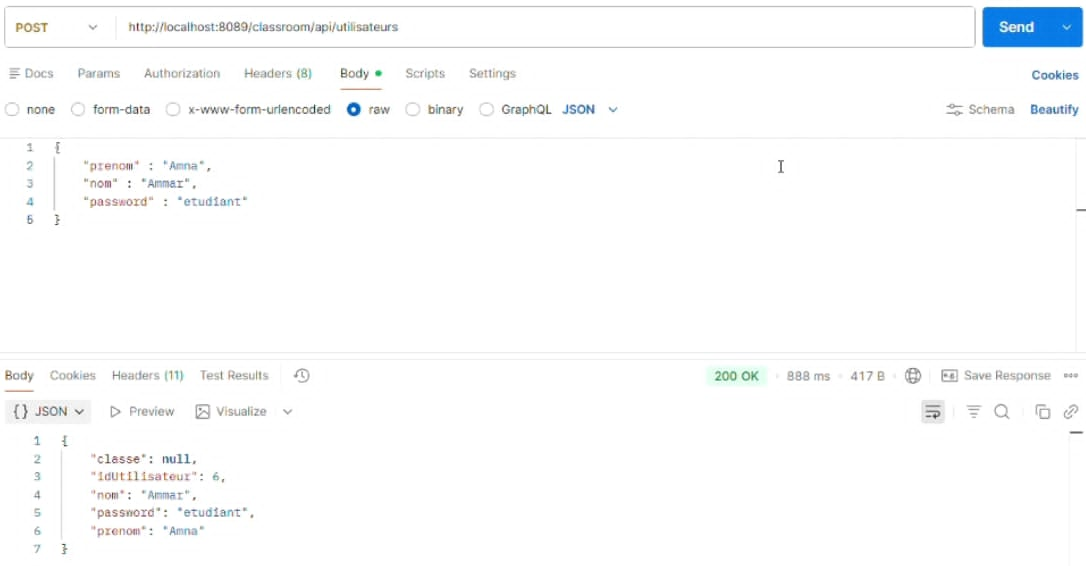
\includegraphics[width=0.9\textwidth]{../diagrams/add_user.jpg}
    \caption{Exécution de la requête d'ajout réussi d'un utilisateur via l'API}
\end{figure}

\subsection{Question 3 : Affectations}
\textbf{Démarche :} Nous avons implémenté la logique métier pour affecter un utilisateur à une classe, et un cours à une classe, en veillant à vérifier l'existence des entités au préalable via les \texttt{Repository}.

\begin{figure}[H]
    \centering
    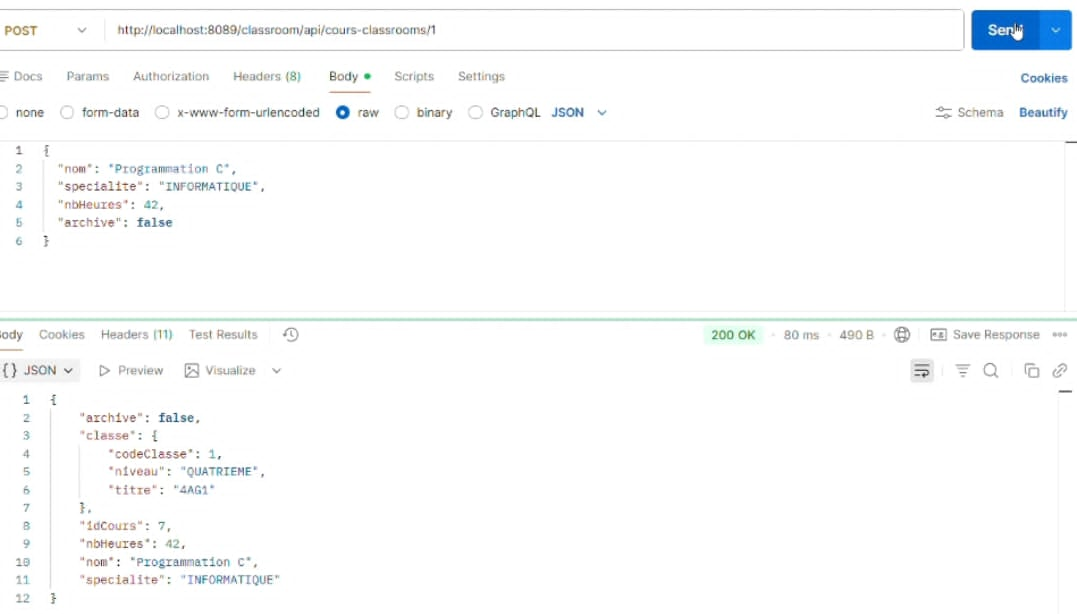
\includegraphics[width=0.9\textwidth]{../diagrams/add_classroom.jpg}
    \caption{Exécution de l'ajout et/ou l'affectation d'un cours (Classroom)}
\end{figure}

\subsection{Question 4 : Nombre d'utilisateurs par niveau}
\textbf{Démarche :} Nous avons exploité la puissance de Spring Data JPA en écrivant une méthode dérivée dans \texttt{IUtilisateurRepository} ou \texttt{IClasseRepository} pour compter les occurrences en fonction de l'énumération \texttt{Niveau}.

\begin{figure}[H]
    \centering
    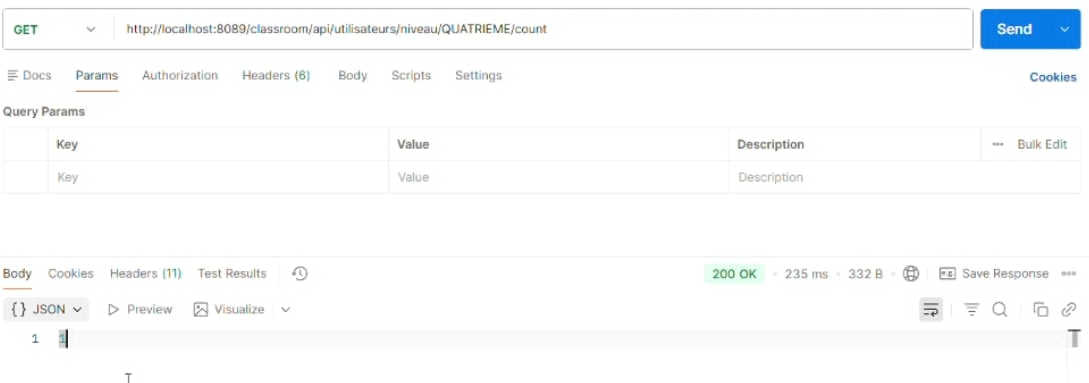
\includegraphics[width=0.9\textwidth]{../diagrams/count_par_niv.jpg}
    \caption{Test de l'endpoint retournant le nombre d'utilisateurs pour un niveau spécifié}
\end{figure}

\subsection{Question 5 : Volume horaire par spécialité et niveau}
\textbf{Démarche :} Cette fonctionnalité complexe a nécessité une requête \texttt{@Query} (JPQL) personnalisée pour effectuer la somme des heures (jointure entre CoursClassroom et Classe).

\begin{figure}[H]
    \centering
    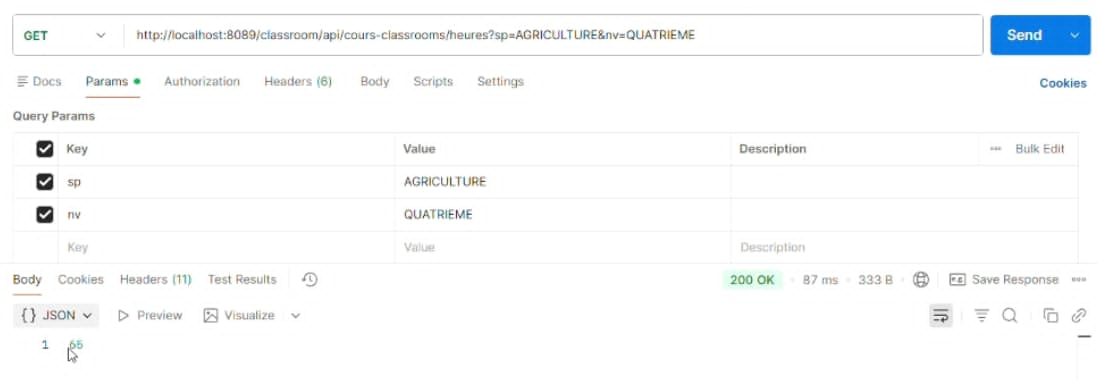
\includegraphics[width=0.9\textwidth]{../diagrams/nb_heures.jpg}
    \caption{Résultat du calcul du volume horaire par spécialité et niveau}
\end{figure}

\subsection{Question 6 : Désaffectation d'un cours}
\textbf{Démarche :} Une méthode spécifique a été créée pour annuler l'affectation d'un cours à une classe (passage de la clé étrangère à \texttt{null} ou retrait de la liste).

\begin{figure}[H]
    \centering
    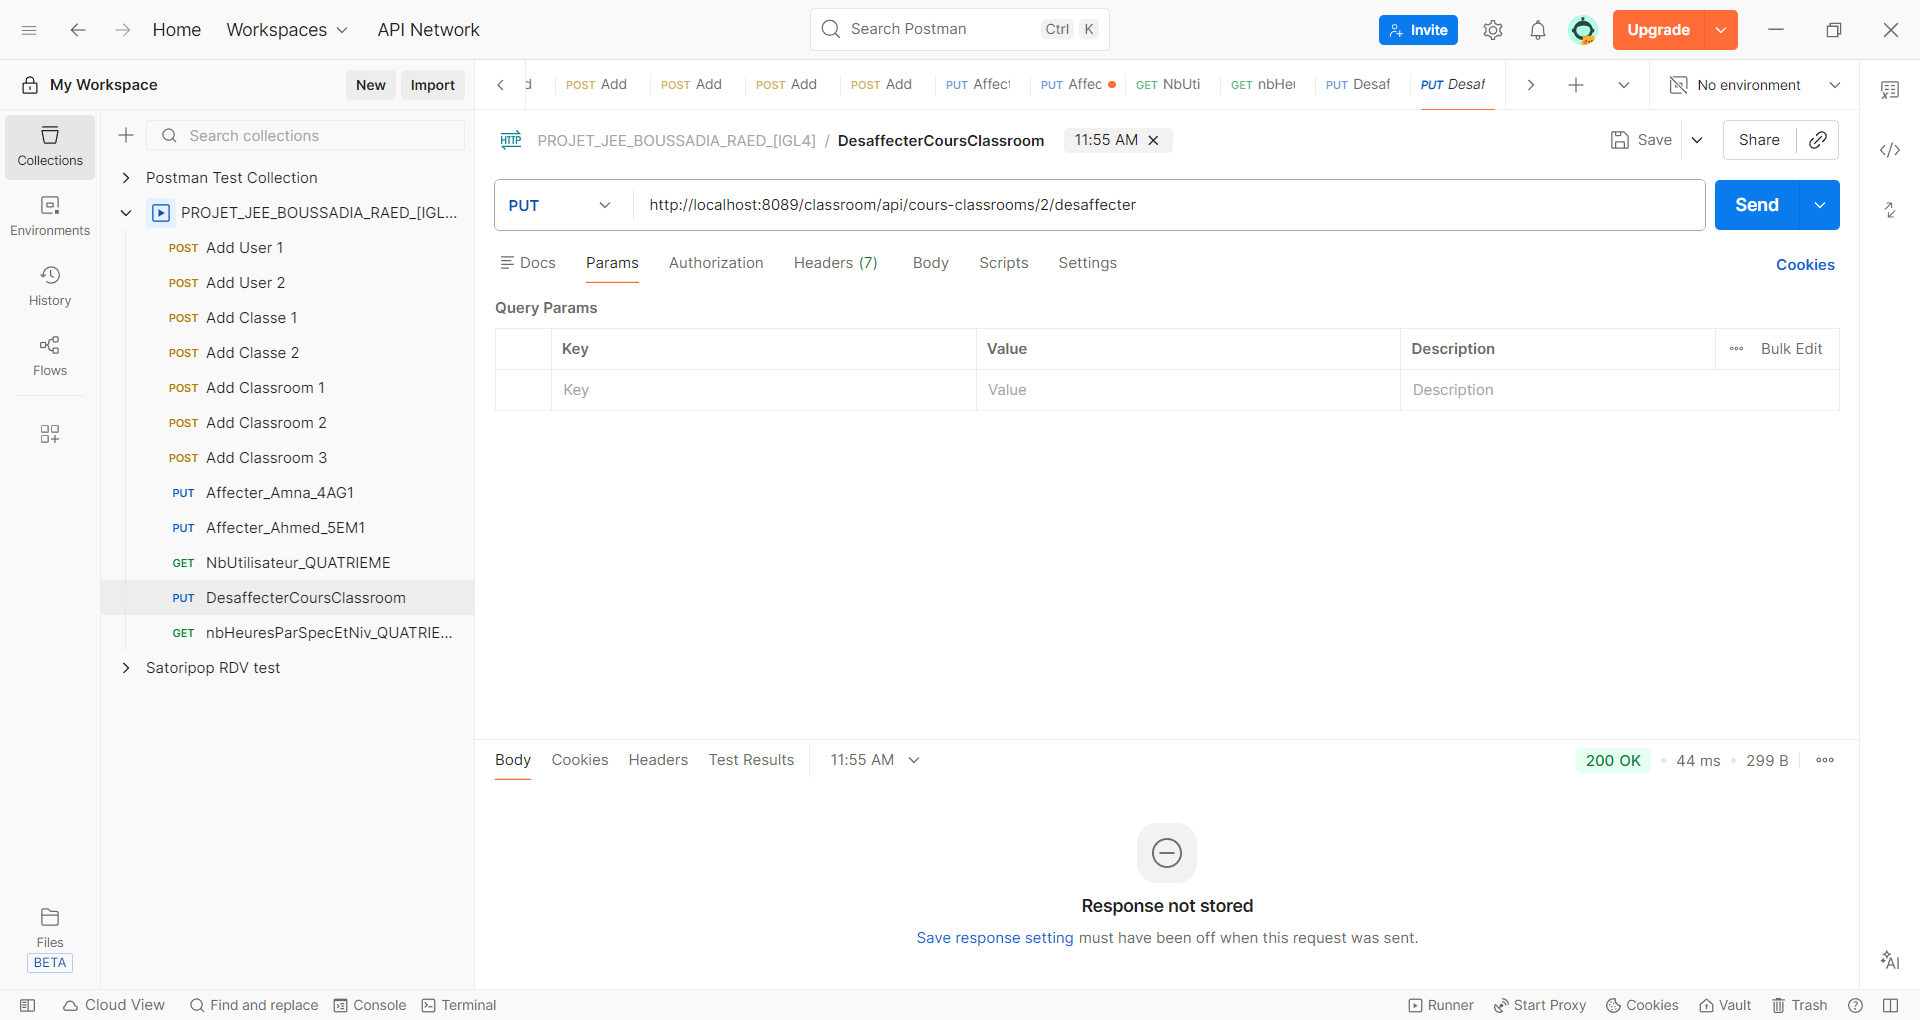
\includegraphics[width=0.9\textwidth]{../diagrams/desaffecter.png}
    \caption{Constat de la désaffectation réussie via l'API}
\end{figure}

\subsection{Question Bonus : Archivage automatique (Spring Scheduler)}
\textbf{Démarche :} Nous avons activé le scheduling avec \texttt{@EnableScheduling} et créé une tâche récurrente (\texttt{@Scheduled(fixedRate = 60000)}) qui bascule tous les cours en état archivé.

\begin{figure}[H]
    \centering
    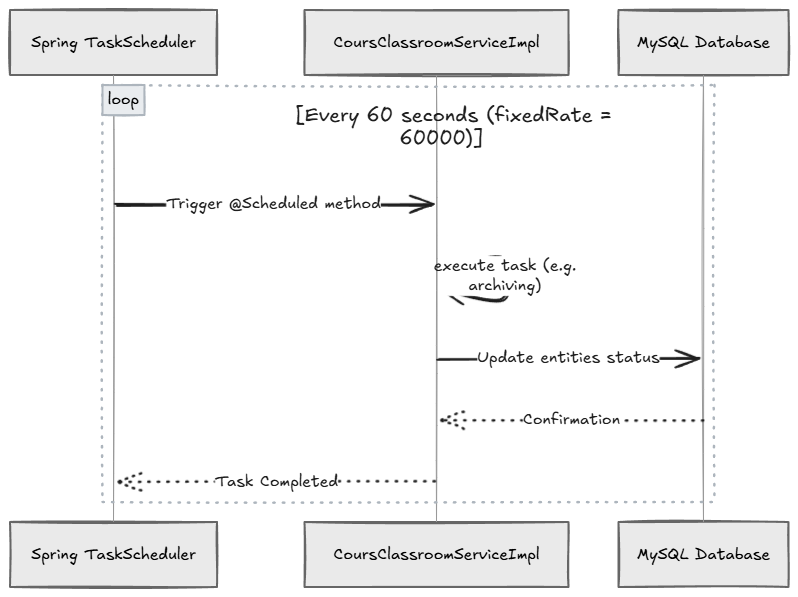
\includegraphics[width=0.7\textwidth]{../diagrams/scheduler.png}
    \caption{Mécanisme d'archivage automatique avec Spring Scheduler}
\end{figure}

\begin{figure}[H]
    \centering
    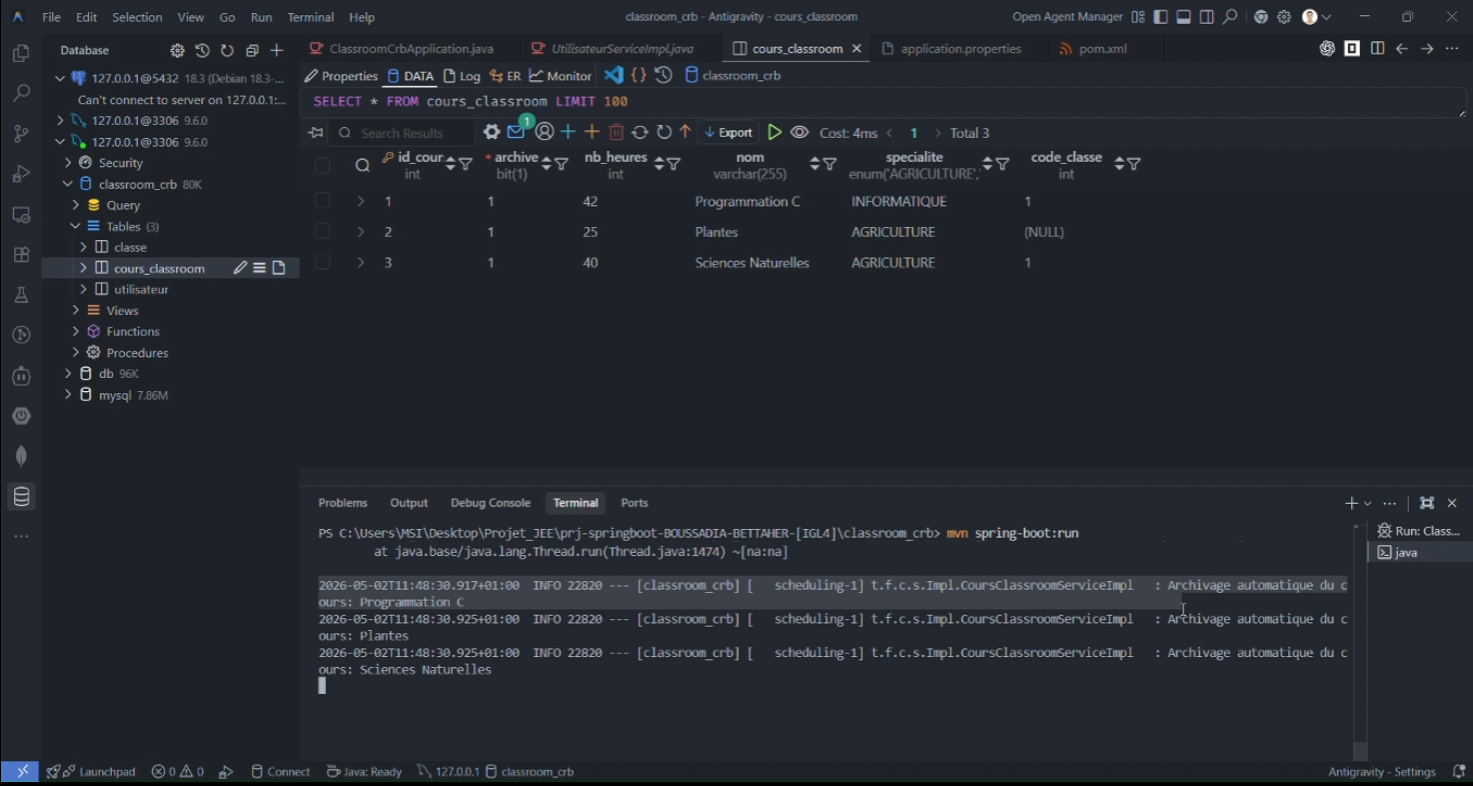
\includegraphics[width=0.9\textwidth]{../diagrams/logs_schedule.png}
    \caption{Logs de la console Spring Boot montrant l'exécution du Scheduler}
\end{figure}

% =========================================================
\section{Interfaces Utilisateur et Interfaces de Test (API)}

Pour valider l'ensemble du projet sans se limiter à des requêtes terminal, nous avons mis en place deux interfaces graphiques.

\subsection{Dashboard UI (Thymeleaf)}
L'interface Thymeleaf offre un rendu web (Server-Side) qui permet de visualiser directement les données de la base.

\begin{figure}[H]
    \centering
    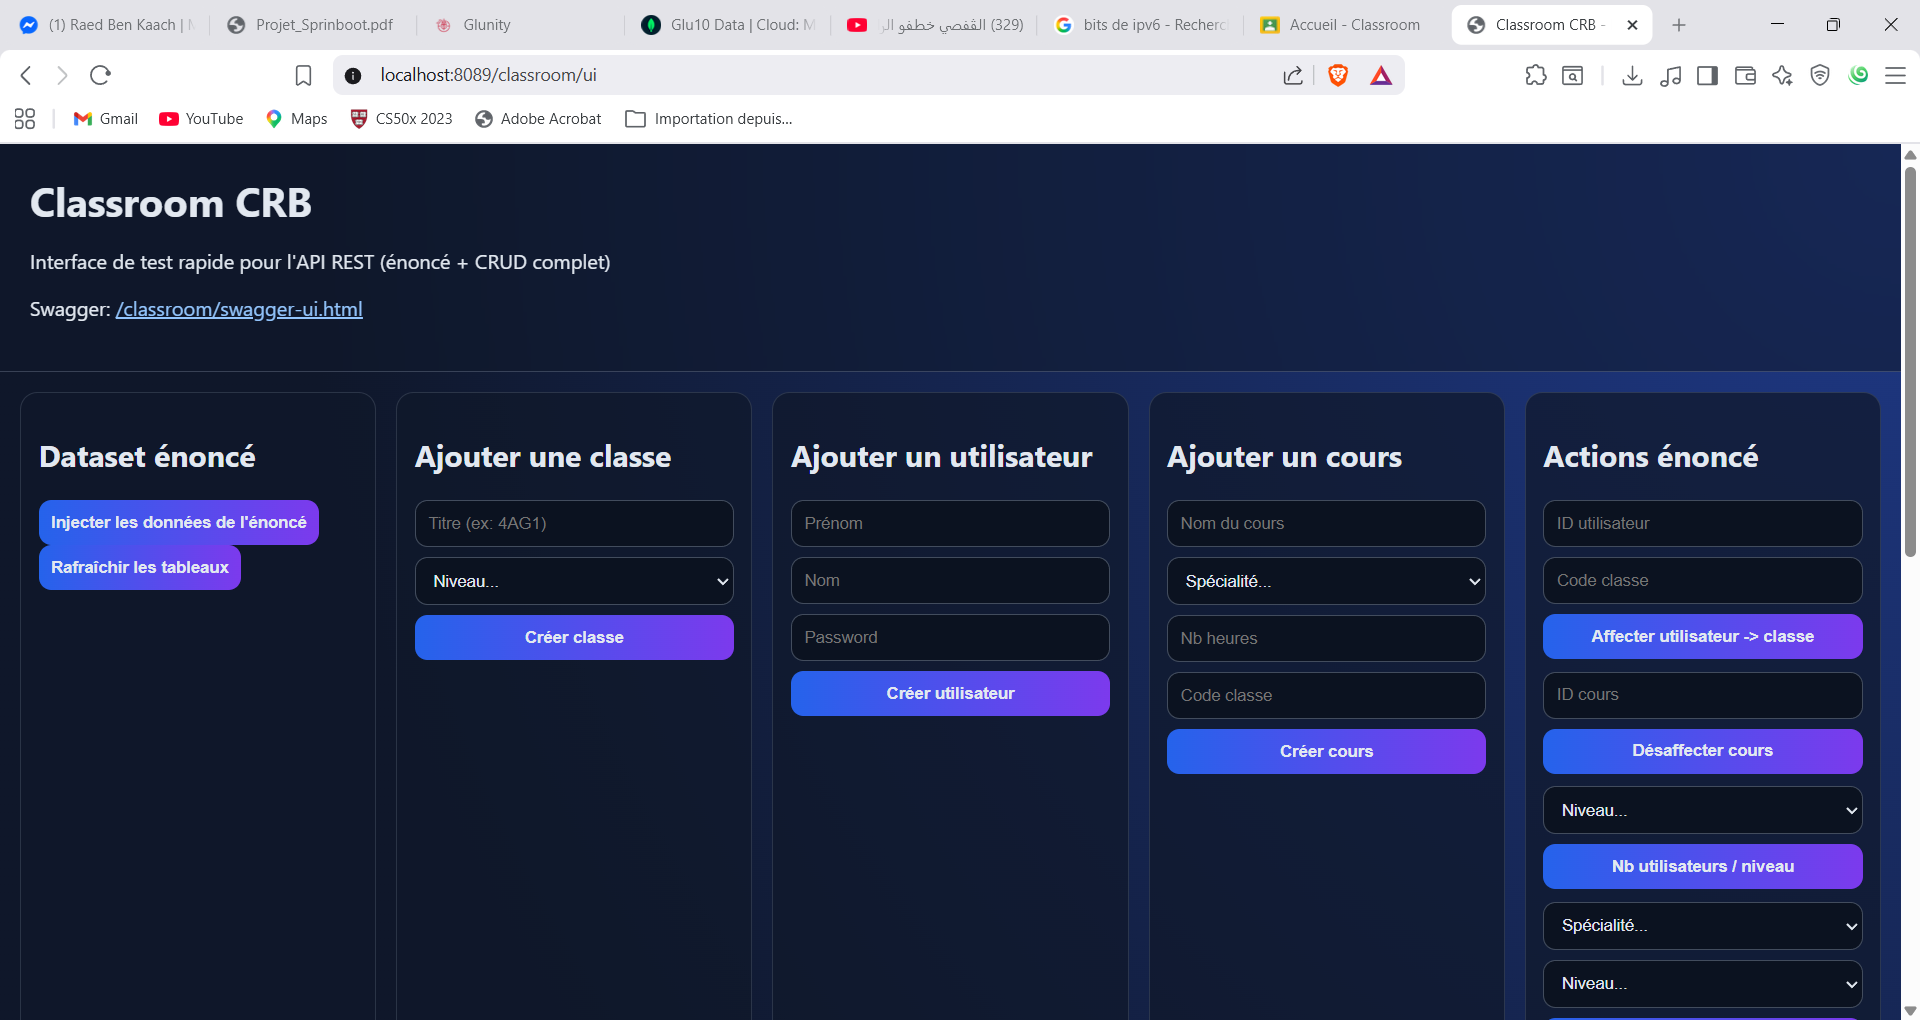
\includegraphics[width=0.95\textwidth]{../diagrams/ui.png}
    \caption{Interface Thymeleaf principale de l'application (Dashboard)}
    \label{fig:ui_dashboard}
\end{figure}

\subsection{Documentation Interactive de l'API (Swagger)}
L'intégration de \textit{Springdoc OpenAPI} génère automatiquement une documentation dynamique, essentielle pour tester individuellement chaque route REST.

\begin{figure}[H]
    \centering
    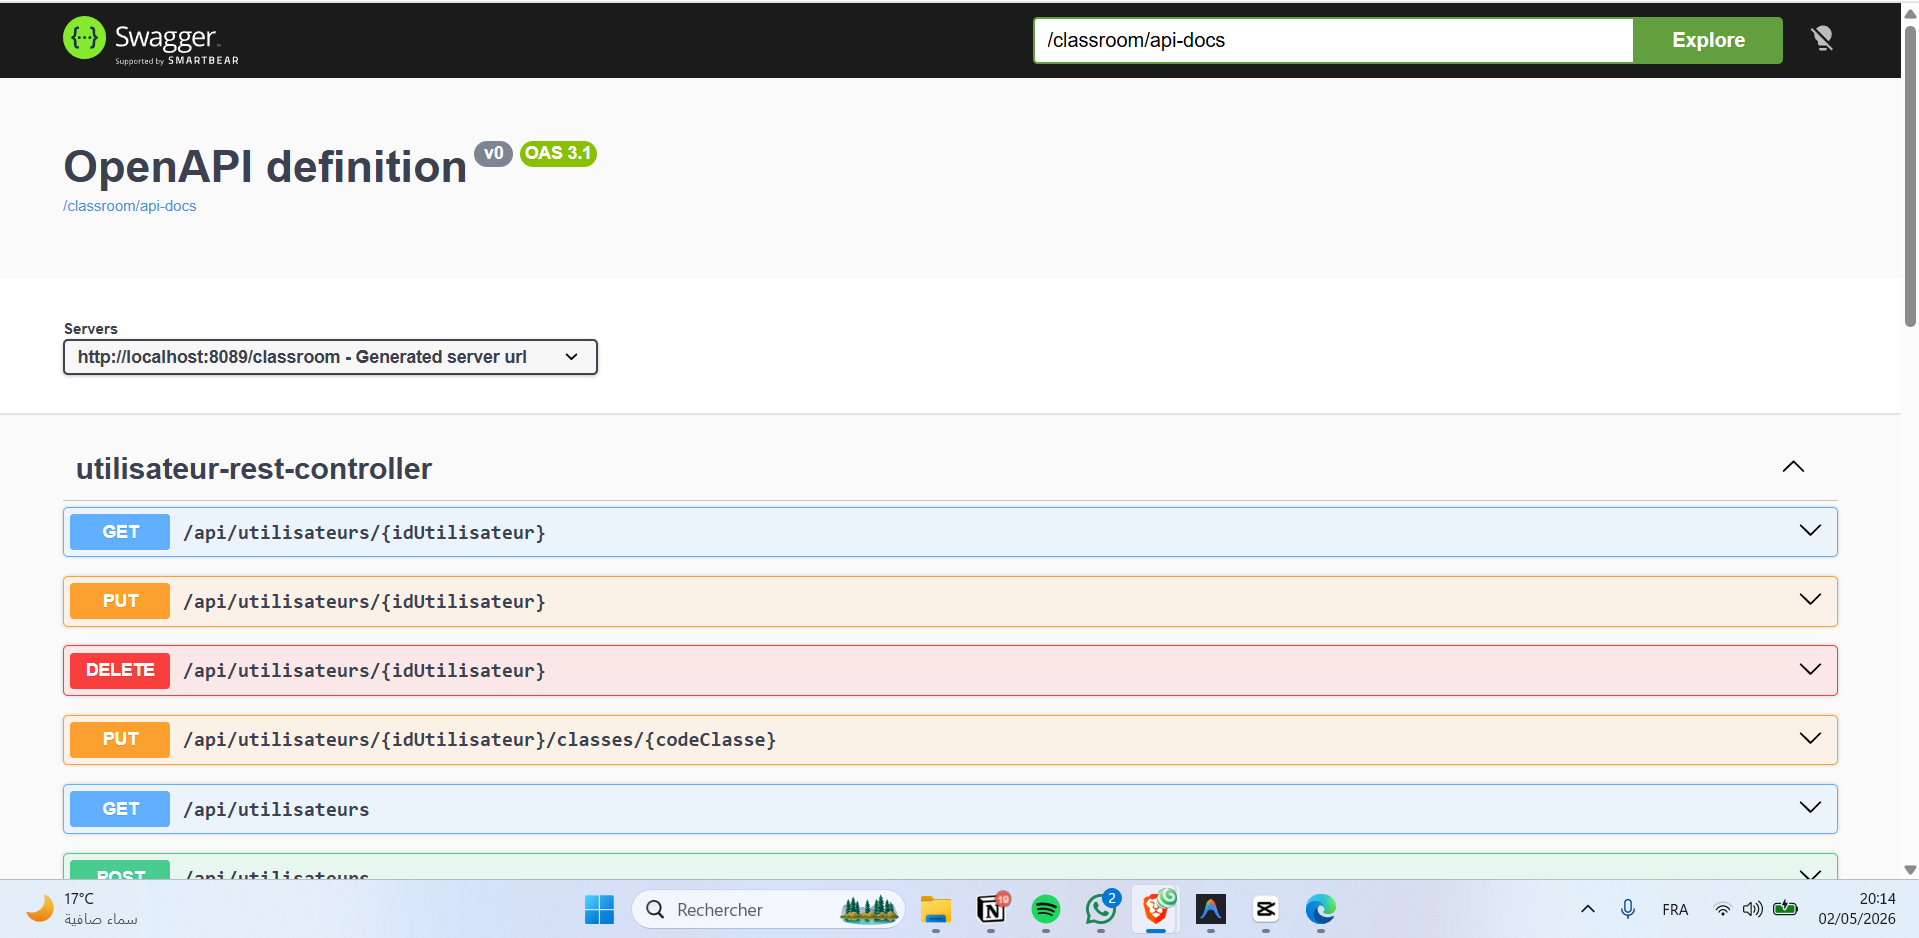
\includegraphics[width=0.95\textwidth]{../diagrams/swagger.png}
    \caption{Interface Swagger de l'application (Liste complète des endpoints)}
    \label{fig:swagger_ui}
\end{figure}

% =========================================================
\section{Déploiement Conteneurisé avec Docker}

Notre projet s'inscrit dans une démarche DevOps moderne en utilisant Docker pour packager l'application.

\subsection{Génération de l'image (Google Jib)}
\textbf{Démarche :} Au lieu d'écrire un fichier \texttt{Dockerfile} manuel, nous avons intégré le plugin Maven \textbf{Google Jib} (visible dans le \texttt{pom.xml}). Ce plugin analyse le projet Java et construit une image Docker optimisée (séparation des classes, ressources et dépendances). L'orchestration avec la base de données MySQL est ensuite pilotée par le fichier \texttt{docker-compose.yml}.

\begin{figure}[H]
    \centering
    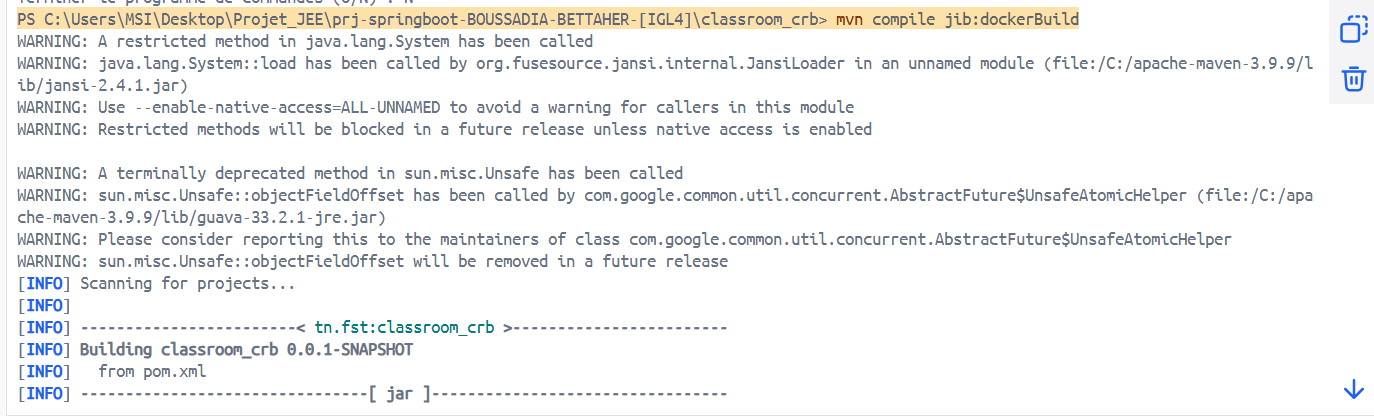
\includegraphics[width=0.9\textwidth]{../diagrams/google_jib.png}
    \caption{Console montrant l'exécution du build via Google Jib}
\end{figure}

% =========================================================
\section{Sécurité et Tolérance aux Pannes (Fault Tolerance)}

Nous avons implémenté des standards de production afin de rendre l'API robuste face aux abus et aux pannes réseau.

\subsection{Sécurité de l'API : Rate Limiting}
\textbf{Démarche :} Afin de prévenir les attaques par déni de service (DDoS) ou le spam de l'API, nous avons mis en place un "Rate Limiter". La configuration définie dans le fichier \texttt{application.properties} limite le nombre de requêtes à 60 par minute par adresse IP. Lorsqu'un client dépasse ce quota, le serveur rejette la demande avec une erreur HTTP \texttt{429 Too Many Requests}.

\begin{figure}[H]
    \centering
    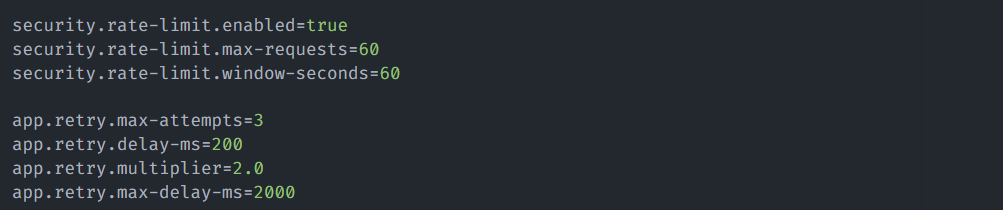
\includegraphics[width=0.9\textwidth]{../diagrams/too_much_requests.png}
    \caption{Requête bloquée avec succès (429 Too Many Requests)}
\end{figure}

\subsection{Tolérance aux pannes : Le Pattern Retry}
\textbf{Démarche :} Pour gérer les micro-coupures de connexion avec la base de données (fréquentes dans les architectures microservices), nous avons activé la tolérance aux pannes avec l'annotation \texttt{@EnableRetry} dans la classe principale \texttt{ClassroomCrbApplication}. L'annotation \texttt{@Retryable} indique à Spring de relancer automatiquement (jusqu'à 3 fois) les méthodes sensibles en cas de \texttt{TransientDataAccessException}, de façon transparente pour l'utilisateur.

% =========================================================
\section{Conclusion}
Ce compte rendu démontre que l'ensemble des questions de l'énoncé ont été traitées, testées et validées (comme en témoignent les captures de notre environnement local). Au-delà de l'énoncé de base, la mise en œuvre d'une architecture physique conteneurisée (Docker/Jib) et l'intégration de mécanismes de sécurité (Rate Limiting) et de résilience (Retry Pattern) dotent le projet "Classroom CRB" d'une dimension professionnelle véritablement prête pour la production.

\end{document}
